%Analyzujte dostupná existující řešení BYOD, zejména z pohledu bezpečnosti.
Tato kapitola se zaměřuje na analýzu existujících řešení na trhu. V první části jsou definovány různé pohledy na BYOD na základě vlastnictví zařízení, typů zařízení a způsobu přístupu do datové sítě. Dále jsou definovány známá technická řešení pro BYOD. Na základě vlastností známých řešení je odděleně zvolen vhodný přístup řešení pro notebooky a mobilní zařízení. Pro tyto přístupy jsou vyhodnoceni nejvýznamnější poskytovatelé. 


 \section{Různé pohledy na BYOD}
 Na problematiku nefiremních zařízení je možné nahlížet z různých úhlů pohledu. V této sekci budou představeny různé možnosti dělení zařízení dle různých kategorií a taktéž budou představeny odpovídající řešení.
 
 \subsection{Rozdělení zařízení podle vlastnictví}
 Na základě toho, kdo je vlastníkem zařízení připojovaného k firemní síti, je určena míra kontroly zařízení firmou.
 
 \subsubsection{Firemní zařízení}
 Jedná se o zařízení, které nakupuje a zároveň spravuje firma. Je ve vlastnictví firmy a pod dohledem IT oddělení. Zařízení plně splňuje politiky firmy a je plně kontrolované.
 
 \subsubsection{Externí firemní}
 Jedná se o firemní zařízení pracovníka externí firmy, jedná se tedy o firemní zařízení, ale jiné firmy. Je tedy pod správou IT oddělení externí firmy.
 
 Zařízení splňuje bezpečnostní politiky externí firmy a je kontrolované externí firmou. Není možné zařízení kontrolovat, je však možné vynutit potřebné bezpečnostní politiky smluvním vztahem s externí firmou.
 
 \subsubsection{Externí soukromé}
 Zařízení externího pracovníka, které není kontrolované firemní politikou externí firmy. Není možné jej kontrolovat a je obtížné vynucovat bezpečnostní politiky.
 
 \subsubsection{Zaměstnanec se soukromým zařízením}
 Vlastní zařízení zaměstnanců. Není kontrolované a může představovat bezpečnostní hrozbu.
 
 \subsection{Rozdělení podle typu zařízení}
 \subsubsection{PC}
 V užším slova smyslu se jedná o osobní počítače s operačním systémem Windows od firmy Microsoft, viz \cite{Intel_Mac_PC}. Windows je aktuálně nejrozšířenější operační systém pro korporátní zařízení. Systém je určený pro zařízení postavená na architektuře x86. Typicky se jedná o stolní počítače a notebooky. Podle statistiky StatCounter \cite{Statcounter1} měl operační systém Windows v únoru 2017 90 procentní podíl na trhu operačních systémů pro desktopy podle počtu přístupů na web. Podle celosvětových statistik přístupů na web v souhrnu všech typů zařízení podle StatCounter má však Windows pouze 38,6 procenta přístupů a mezi běžnými uživateli je zřejmá tendence v upřednostňování jiných zařízení na úkor PC \cite{HNAndroid}.
 
\begin{figure}[h!]
%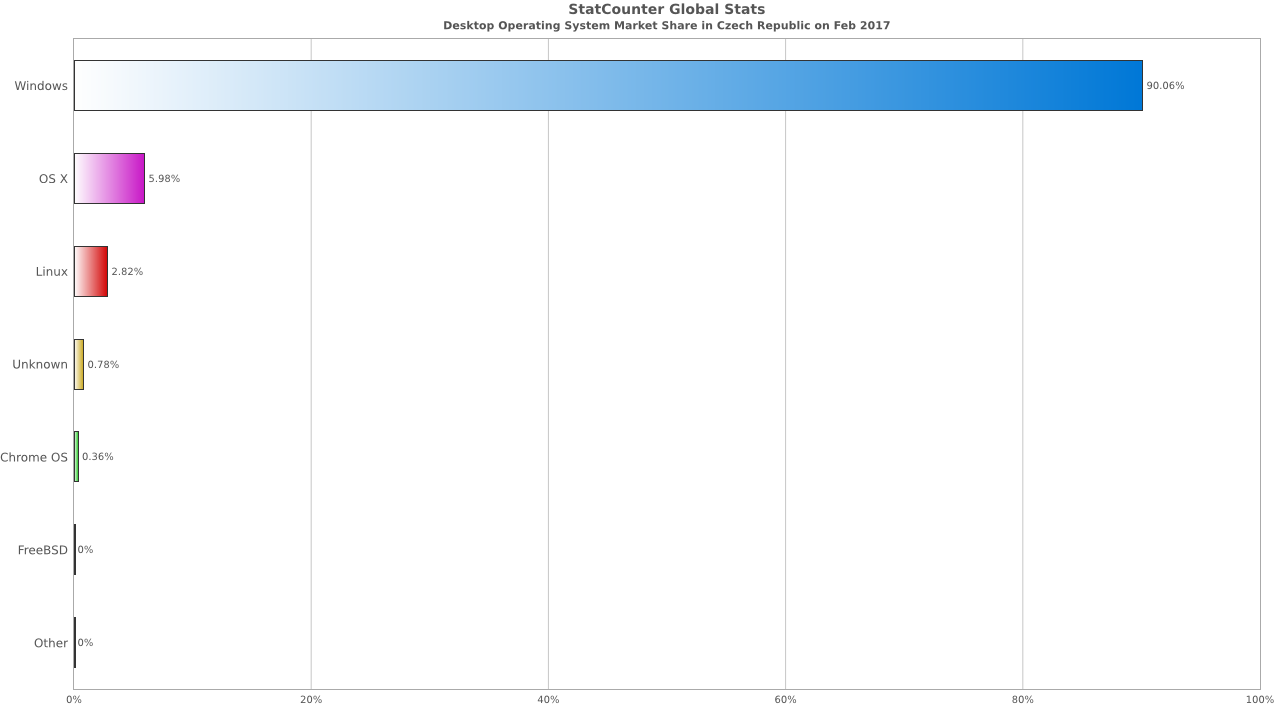
\includegraphics[width=13cm]{img/StatCounter_Desktop}
\centering
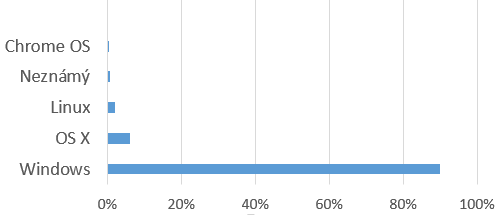
\includegraphics[width=10cm]{img/1_Desktopy_CZ}
\caption{Statistika podílu operačních systémů pro desktopy v České republice podle přístupů na web. Převzato z \cite{Statcounter1}.} 
\centering
\end{figure}
 
 
 
 \subsubsection{Mac}
 Počítač s operačním systémem MAC OS \cite{AppleMacOS}. Jedná se o proprietární operační systém pro počítače firmy Apple. Podle StatCounter je jeho podíl na trhu mezi desktopovými operačními systémy podle počtu přístupů na web v České republice necelých šest procent. Populární je zejména ve Spojených státech, kde se jeho podíl mezi desktopovými operačními systémy podle metodiky StatCounteru pohybuje okolo dvaceti procent.
 
\begin{figure}[h!]
%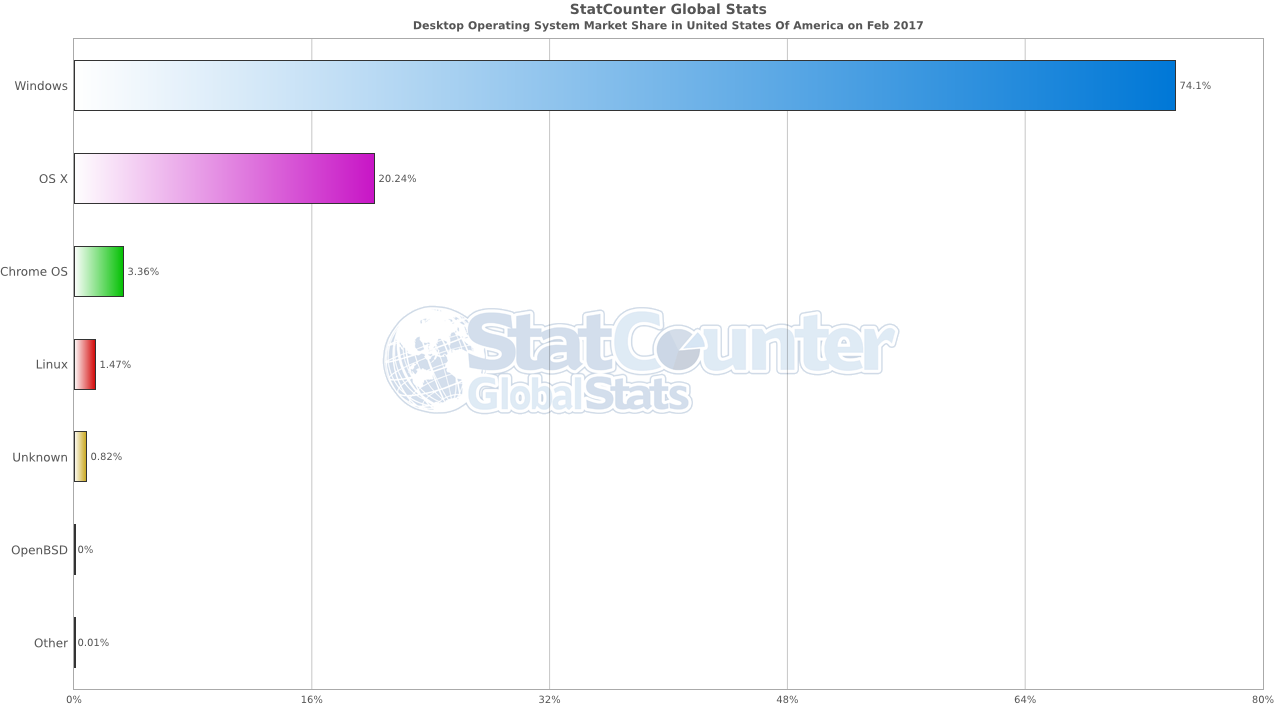
\includegraphics[width=13cm]{img/StatCounter_Destop_USA}
\centering
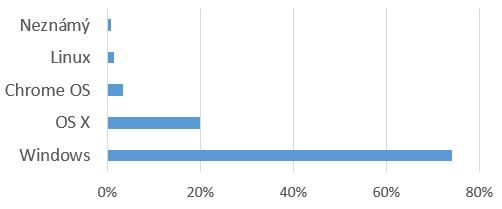
\includegraphics[width=10cm]{img/2_Desktopy_US}
\caption{Statistika podílu operačních systémů pro desktopy v USA podle přístupů na web. Převzato z \cite{Statcounter1}} 
\centering
\end{figure}%\todo{citace}
 
 
 \subsubsection{Chytrý telefon či tablet}
 Podle společnosti Gartner \cite{GartnerSmartphone} je chytrý telefon definován jako mobilní komunikační zařízení používající identifikovatelný otevřený operační systém. Tento systém je podporován aplikacemi třetích stran od komunity vývojářů. Aplikace třetích stran mohou být instalovány nebo odstraněny a mohou být vytvořeny přímo pro operační systém zařízení a aplikační programové rozhraní, případně pro oddělenou vrstvu jakou může být například Java. Operační systém musí podporovat multitaskingové prostředí a uživatelské rozhraní, které dokáže obsloužit více aplikací najednou. Například zobrazení emailu během přehrávání hudby.
 
  \begin{figure}[h!]
%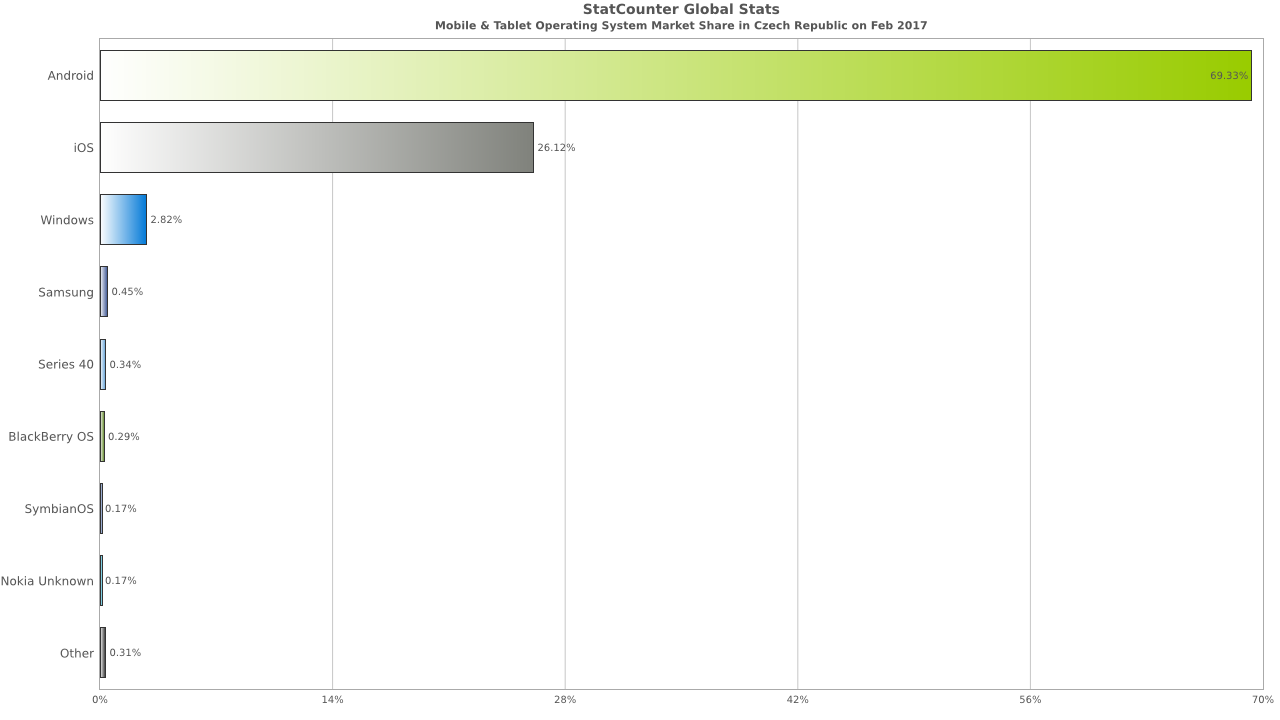
\includegraphics[width=13cm]{img/StatCounter_MobileBar}
\centering
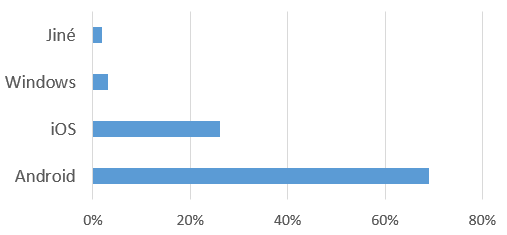
\includegraphics[width=10cm]{img/3_Mobil_CZ}
\caption{Statistika podílu operačních systémů pro mobilní zařízení v České republice podle přístupů na web. Převzato z \cite{Statcounter1}.} 
\centering
\end{figure}
 
 Obecněji se jedná o mobilní zařízení s možností instalace aplikací. V současné době jsou nejpopulárnější zařízení s operačním systémem Android od firmy Google a iOS od firmy Apple. V České republice je podle metodiky měření společnosti StatCounter pro únor 2017 nejpopulárnější operační systém Android s podílem 68 procent. Operační systém iOS je na drůhém místě s podílem 26 procent. Více než jednoprocentní podíl má již pouze Windows s necelými čtyřmi procenty \cite{HNAndroid}. 
 

 
Celosvětově je zřejmá rostoucí obliba mobilních zařízení mezi uživateli, a to především na úkor klasických PC s operačním systémem Windows. Vzhledem k postupné změně návyků uživatelů je vyžadováno, aby firemní prostředí na tento trend vhodně reagovalo. 


\begin{figure}[h!]
%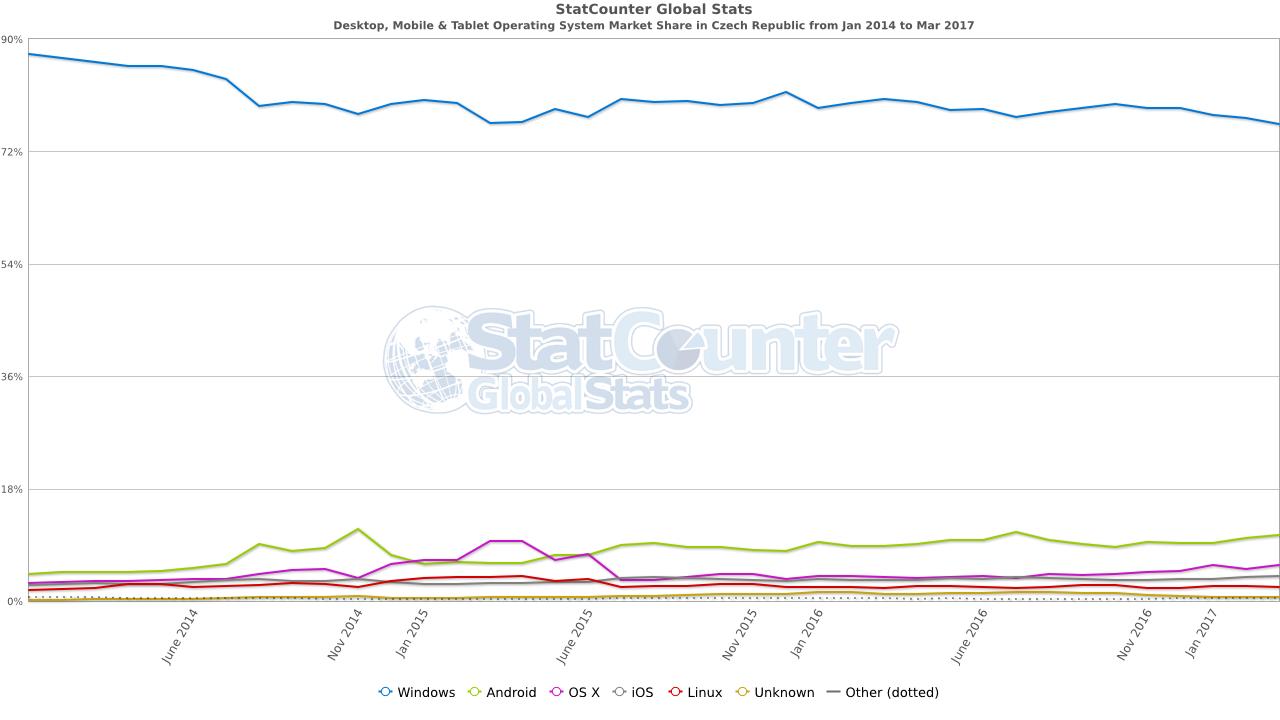
\includegraphics[width=13cm]{img/StatCounter_VyvojVse}
\centering
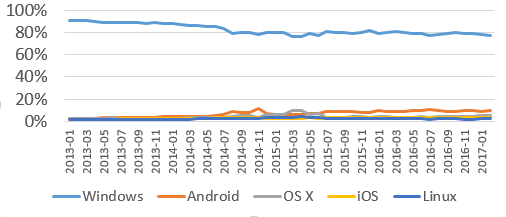
\includegraphics[width=13cm]{img/4_vyvoj_vse_CZ}
\caption{Statistika vývoje podílů všech operačních systémů v České republice podle přístupů na web. Převzato z \cite{Statcounter1}.} 
\centering
\end{figure}

\begin{figure}[h!]
%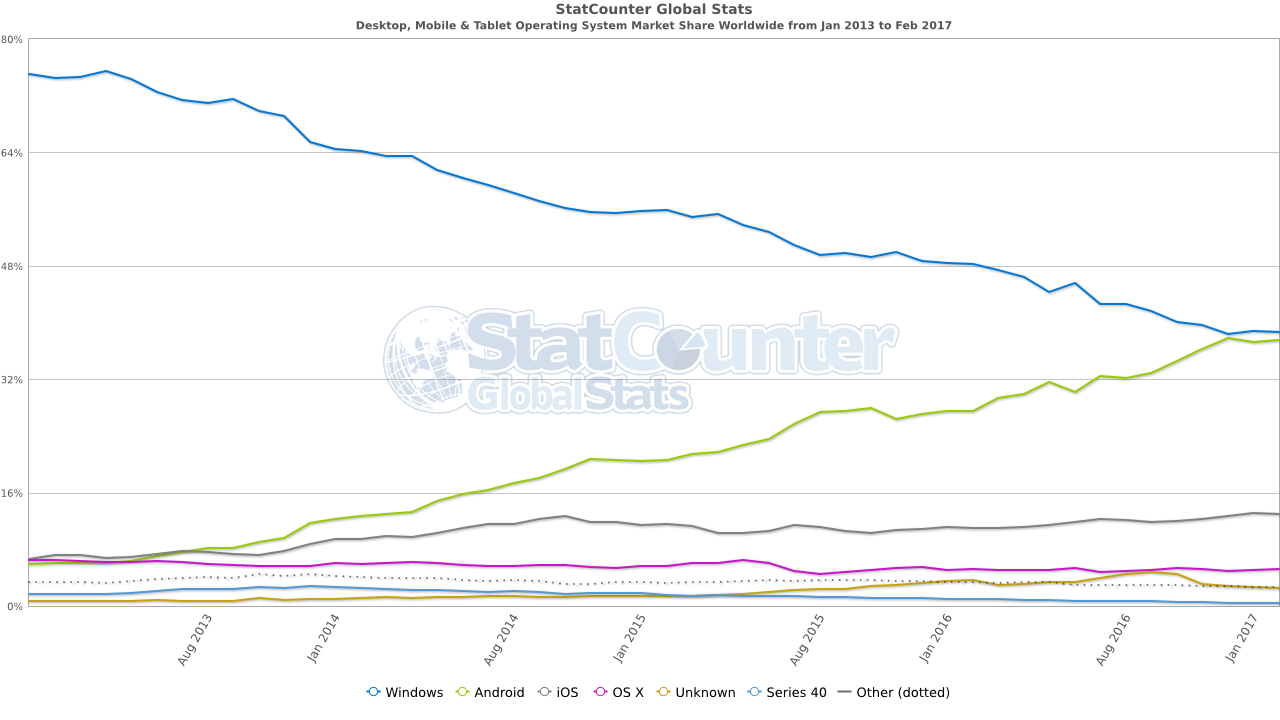
\includegraphics[width=13cm]{img/StatCounter_All_Worldwide}
\centering
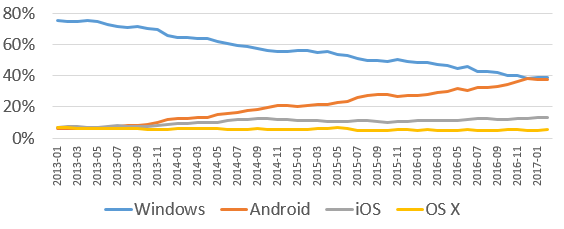
\includegraphics[width=13cm]{img/5_vyvoj_vse_global}
\caption{Statistika vývoje podílů všech operačních systémů celosvětově podle přístupů na web. Převzato z \cite{Statcounter2}.} 
\centering
\end{figure}
 
U těchto zařízení se nepředpokládá nutnost přístupu k podnikovým aplikacím, ale je vyžadován okamžitý přístup k emailům, kontaktům či dokumentům, a to nezávisle na místě použití.

Dle reportu od společnosti Nokia Thread Intelligence Lab \cite{Nokia2, Nokia1}, který monitoroval aktivitu malwaru v sítích mobilních operátorů mezi lety 2012 a 2015 měly 60 \% veškeré aktivity malwaru v mobilních sítích na svědomí chytré telefony, zbytek šel na vrub Windows PC.

V prosinci 2015 vykazovalo známky napadení škodlivým softwarem 0,3 \% všech chytrých telefonů. Nejvíce napadení zaznamenala zařízení s operačním systémem Android, ovšem na seznam s dvaceti nejčastěji se vyskytujícími druhy škodlivého software se dostali i dva zástupci pro operační systém iOS (XcodeGhost a Flexispy). V říjnu 2015 bylo 6 \% všech napadených zařízení značky iPhone.
 
 
 %%%%%%%%%%%%%%%%%%%%%%%%%%%%%%%%%%%%%%%%%%%%%%%%%%%%%%%%%%%%%%%%%%%%%%%%%%%%%%%%%%%%%%%%%%%%%%%%%%%%%%%%%%%%%%%%%%%%%%%%%%%%%%%%%%%
 \subsection{Rozdělení podle typu přístupu do datové sítě}
 \subsubsection{Ethernet}
 Jedná se o pevné připojení do sítě pomocí kabelu \cite{pcmagEthernet}. Je vhodné pro firemní počítače, není vhodné pro zařízení typu mobilní telefon či tablet.
 
 Je definované ve standardu IEEE 802.3.
 
 \subsubsection{WiFi}
 
 Bezdrátové připojení pomocí WiFi sítí. Jedná se o standardní technologii pro bezdrátové sítě WLAN \cite{pcmagWifi}. Tento typ připojení je vhodný pro přenosné počítače, mobilní telefony i tablety. WiFi je definováno standardem IEEE 802.11.
 
 \subsubsection{VPN}
 
 Virtual private network čili vzdálené připojení do firemní sítě. Hlavním smyslem VPN je vytvořit soukromou síť pomocí tunelování a nebo šifrování skrze veřejný internet tak, aby uživatelé mohli vzdáleně přistupovat ke službám dostupným pouze zevnitř sítě \cite{ciscoJournal}.
 
 
 %%%%%%%%%%%%%%%%%%%%%%%%%%%%%%%%%%%%%%%%%%%%%%%%%%%%%%%%%%%%%%%%%%%%
 
 
 
 \section{Známé způsoby řešení BYOD}%\todo{Zejmena z pohledu bezpecnosti}


\subsection{Virtualizace} 
Podle \cite{Shackleford} je virtualizace abstrakcí výpočetních zdrojů od fyzické hardwarové vrstvy. Virtuální stroj vystupuje jako samostatný výpočetní systém dostupný z jiného stroje. Díky virtualizaci je možné oddělit data a prostředí fyzického a virtuálních strojů. Jako hostitel je nazývána platforma na které běží hypervizor. Virtuální stroj je pak systém na kterém běží virtuální prostředí. Reprezentuje kompletní hardwarovou platformu. Virtuální stroje pak běží nad hypervizorem. 

Hypervizor je hlavní komponenta virtualizece. Rozeznáváme 2 druhy:

\subsubsection{Hypervizor typu 1}
Hypervizory prvního typu jsou nainstalovány přímo nad hardware. Mezi hardware a virtuálními stroji s operačními systémy tak není žádná další vrstva. Hypervizory typu 1 jsou zpravidla instalovány na servery ve výpočetních střediscích.

\begin{figure}[h!]
\centering
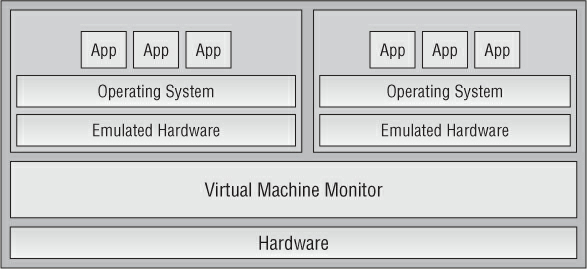
\includegraphics[width=10cm]{img/shackleford1}
\caption{Schéma virtualizace s hypervizorem typu 1. Převzato z \cite{Shackleford}.} 
\end{figure}

\subsubsection{Hypervizor typu 2}
Hypervizory druhého typu jsou aplikace instalované v rámci existujícího operačního systému. Mezi hardware a operačními systémy virtuálních strojů je tak navíc vrstva operačního systému hostitelského stroje. Hypervizory typu 2 jsou zpravidla instalovány na pracovní stanice.

\begin{figure}[h!]
\centering
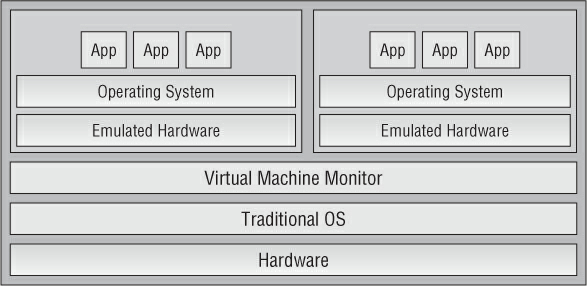
\includegraphics[width=10cm]{img/shackleford2}
\caption{Schéma virtualizace s hypervizorem typu 2. Převzato z \cite{Shackleford}.} 
\end{figure}

\subsection{Hrozby spojené s virtualizací}
Hlavní výhodou virtualizace je oddělení jednotlivých prostředí. Samotnou virtualizací se však bezpečnost nezvyšuje a ve virtualizovaném prostředí existují stejné hrozby jako v prostředím fyzickém. Z hlediska BYOD je však právě oddělení prostředí tou zásadní vlastností, jelikož úroveň zabezpečení firemního virtuálního stroje lze odděleně spravovat.

Kniha \cite{Shackleford} identifikuje několik hrozeb spojených s provozem virtuálních strojů. Relevantní pro tuto práci jsou:

\begin{description}
  \item[Škodlivý software] Byly objeveny některé druhy škodlivého softwaru, které dokáží detekovat, že se nachází ve virtualizovaném prostředí. Díky tomu dokáží modifikovat svoje chování a lépe se tak maskovat.
  \item[Únik z virtuálního stroje] Podle \cite{Shackleford} zatím nebyl zaznamenán takový útok, kdy by kódu běžícímu uvnitř virtuálního stroje podařilo dostat ven a ohrozit tak hostitelský systém nebo jiný virtuální stroj. Koncept toho druhu útoků byl však několikrát dokázán v laboratorních podmínkách. Pro tyto koncepty je však nutné připravit jak software uvnitř hostitelského tak virtualizovaného systému, nebo využít některou z funkcí klienta pro sdílení mezi hostitelským a virtualizovaným systémem.
  \item[Další zranitelnosti] Chyby v softwaru pro virtualizaci mohou znamenat například možnost vzdáleného vyřazení stanice z provozu, spuštění škodlivého kódu nebo dalších útoků. Zranitelnosti jsou předmětem bezpečnostních záplat.
\end{description}

 \subsection{Centralizovaná virtualizace}
 Pod pojmem centralizovaná virtualizace se rozumí běh virtuálních strojů na serveru ve výpočetním středisku. Používají se tedy hypervizory typu 1. Klienti k těmto virtuálním strojů přistupují vzdáleně pomocí technologie VDI. Nejsou tedy spotřebovávány výpočetní prostředky klienta, ale je zapotřebí kvalitní konektivita do výpočetního střediska.
 
 Nejznámějšími zástupci centralizované virtualizace jsou: Microsoft remote desktop, VMWare Horizon, Citrix XenDesktop.
 
 \subsection{Distribuovaná virtualizace}
 Pojmem distribuovaná virtualizace se rozumí běh virtuálních strojů přímo na koncových stanicích uživatelů.  Používá se tedy hypervizor typu 2. Spotřebovávají se tedy výpočetní prostředky stroje klienta, není však obecně potřeba konektivita s vnějším světem.
 
 Nejznámějšími zástupci jsou: Oracle Virtualbox, VMWare Fusion, VMWare Workstation, VMWare Player, VMWare Horizon Flex, Parallels Desktop.
 
 
 \subsection{DaaS}
 Desktop as a service je variace na centralizovanou virtualizaci. Výpočetní středisko však není uvnitř společnost, ale vlastní jej externí subjekt. Ten pak jednotlivé pracovní stanice pronajímá formou pravidelných poplatků za službu. Pro IT oddělení tak odpadají náklady na správu serverů, síťové infrastruktury a dalších souvisejících opatření. Tento model není pro zkoumanou společnost vhodný, jelikož firemní data by se nacházela mimo společnost a docházelo by tak k ohrožení firemních aktiv.
 
 Nejznámější poskytovatelé jsou: VMWare Horizon Air, Citrix XenDesktop, Amazon Work Spaces.
 
  \subsubsection{Virtualizace aplikací}
 Další možností je nevirtualizovat celý operační systém, ale pouze aplikace. Mezi výhody patří snadná aktualizace aplikací, snadná správa přístupu k aplikacím či nenáročnost na výpočetní výkon klienta. Data a přístupy je takto však možné oddělit pouze v rámci takto nasazených aplikací.
 
 Mezi hlavní nevýhody patří problémy s periferiemi jako např. tiskárny či nutnost stálé a kvalitní konektivity.
 
  Nejznámějšími zástupci služeb pro virtualizace aplikací jsou: Citrix XenApp, VMware Horizon, Dell vWorkspace, and Microsoft RDSH.
  
  
  \subsubsection{Používání webových aplikací}
  Variací na virtualizaci aplikací je jejich úprava pro přístup z webového prohlížeče. To však není možné u všech používaných aplikací ve zkoumané společnosti.
  
 \subsection{Rozlišení na úrovni sítě}
 Použitím Network Access Controll neboli NAC je možné spravovat přístup zařízení do sítě. Je možné nastavit autentifikační kontroly a další bezpečnostní politiky, které musí zařízení splňovat aby bylo do sítě vpuštěno. 
 
 Společnost Gartner identifikuje několik funkcí, které tato řešení nabízejí \cite{GartnerNAC}. Politiky mohou pojmout různé fukce jako například autentifikaci zařízení, autorizaci uživatele, lokaci, čas či přístup k aplikacím a zdrojům.
 
 Dále je možné posoudit stav zařízení z hlediska aktuálnosti systému a antivirových definic co se týče zařízení s Windows, nebo přítomnost EMM, viz \ref{EMM},  na mobilních zařízení.
 
 Přístup je přidělován pomocí síťové infrastruktury s použitím 802.1X protokolu, virtuálních LAN, či seznamů pro řízení přístupů neboli ACL (Access Control List).
 
 Dalšími službami poskytovanými NAC řešeními může být vytváření sítí pro hosty, monitoring připojených zařízení či integrace s dalšími bezpečnostními prvky.
 
 
Gartner ve své studii \cite{GartnerNAC} zmiňuje následující prudukty: Aruba ClearPass, Auconet BICS, Brandford Networks Network Sentry, Cisco ISE, Extreme Networks ExtremeControll, ForeScout CounterACT, Impulse Point SafeConnect, Info Express CGX, Portnox CLEAR, Pulse Policy Secure, SnoopWall Netshield.
 
 

 
 
 \subsubsection{EMM/EMS}\label{EMM}
 Enterprise mobility management nebo též Enterprise Mobility suite umožňují integrovat a spravovat mobilní zařízení v rámci firemní infrastruktury.
 Dle agentury Gartner jsou EMM balíky lepidlem, které připojuje mobilní zařízení do firemní infrastruktury. \cite{Gartner_EMM_2016}
 
 EMM mají následující funkce:
 \begin{itemize}
     \item nastavují zařízení a aplikace pro nasazení ve firemním prostředí
     \item sledují dodržení firemních politik a spravují firemní aktiva
     \item snižují riziko ztráty dat, krádeže či dalších incidentů řízením šifrování dat, přístupových práv, sdílených zařízení, obalováním aplikací či zamknutím zařízení.
     \item umožňují vzdálenou podporu zařízení pro IT oddělení
 \end{itemize}
 
Výzkum společnosti J Gold Associates z roku 2016 \cite{JBBrief} 
ukazuje, že firmy v drtivé většině nenasazují všechny funkce, které EMM řešení nabízejí. Nejpoužívanější funkce EMM jsou vypsány na obrázku (\ref{funkceEMM}) 

\begin{figure}[h!]
\centering
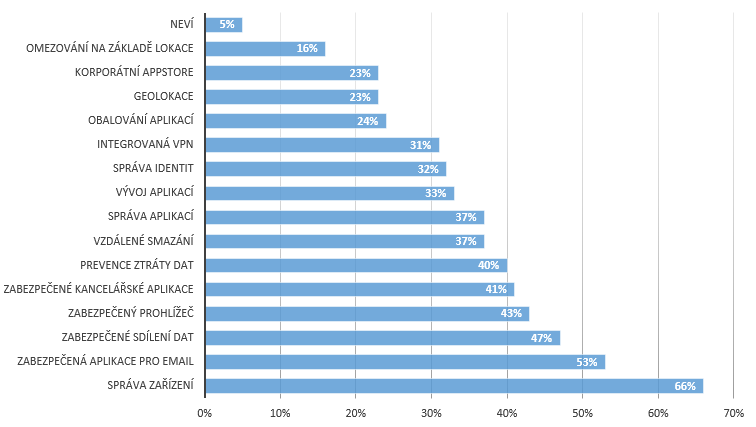
\includegraphics[width=13cm]{img/funkceEMM}
\caption{Které komponenty EMM řešení organizace zapojené do průzkumu aktuáně používají? Převzato z \cite{JBBrief}.} 
\end{figure}\label{funkceEMM}

 
 
 
  \subsection{MDM}
 Mobile device management je software pro správu mobilního zařízení. Je podmnožinou EMM. Mezi základní funkce tohoto software podle \cite{systemOnline} patří:
 \begin{itemize}
     \item Automatické nastavení mobilního zařízení. Umožňuje IT oddělení nastavit zařízení podle firemních potřeb. To zahrnuje instalaci bezpečnostních certifikátů, nastavení uživatelských účtů či dalších nastavení umožňující přístup k firemní síti.
     \item Možnost vzdáleného vymazání. Umožňuje vzdáleně vymazat data tak, aby nebyla dostupné. To je užitečné v případě ztráty či krádeže zařízení, nebo po ukončení pracovního poměru se zaměstnancem.
     \item Vynucení bezpečnostních politik. To zahrnuje vynucení silného hesla, šifrování dat či omezení některých funkcí, například propojení se soukromým cloudovým úložištěm. 
     \item Detekce jailbreak/root zařízení. Detekuje spuštění zařízení v administrátorském režimu, což je ve firemním prostředí nepřípustné.
     \item Blacklisting/whitelisting aplikací. Umožňuje správci zařízení zvolit, které aplikace je a není možné instalovat.
     \item Monitoring. Umožňuje sledovat přístupy uživatele k jednotlivým službám.
     \item Administrace. Umožňuje hromadné aktualizace, instalace či odinstalace aplikací pro zařízení ve firemní flotile.
 \end{itemize}
 

 
 \subsection{MAM} 
 Mobile application management. MAM je též podmnožinou EMM. Narozdíl od MDM nespravuje zařízení jako celek, ale pouze podnikové aplikace. Tyto aplikace jsou získávány přes speciální obchod s aplikacemi. Podle \cite{MAMcitace} mezi hlavní funkce MAM patří:
 \begin{itemize}
     \item Podnikový obchod s aplikacemi. Umožňuje nasazování vlastních i komerčních aplikací pro potřeby businessu.
     \item Podpora správy a distribuce aplikací s užitím API operačního systému či hromadného nákupu aplikací.
     \item Kontejnerizace aplikací
     \item Reporting o užívání aplikací
 \end{itemize}
 
 Podle \cite{Gartner_EMM_2016} jsou pomocí MAM běžně uplatňovány následující politiky:
 \begin{itemize}
     \item Vyžadování iniciace VPN spojení pro aplikaci při spuštění
     \item Šifrování podnikových dat (často s použitím silnějšího šifrování než by bylo použito v rámci operačního systému)
     \item Omezení sdílení dat mezi aplikacemi pouze na podnikové aplikace
     \item Omezení copy/paste funkcionality
     \item Vyžadování specifického stavu při spuštění nebo při přístupu -- například nebyl detekován root nebo jailbreak
 \end{itemize}
 
  
%\begin{figure}[h]
%\centering
%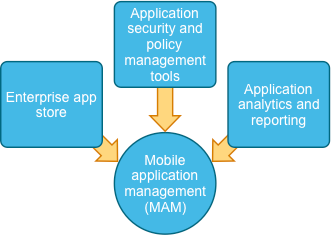
\includegraphics[width=7cm]{img/MAM-Offering}
%\caption{Gartner Magic quadrant. Převzato z } 
%\label{MAM:nacrt}
%\end{figure}\todo{ citace https://www.ibm.com/developerworks/community/blogs/mobileblog/entry/got\_mam\_mobile\_application\_management\_in\_your\_2013\_mobile\_menu25?lang=en}


\subsection{MCM} 
Mobile content management. Jedná se o software pro správu obsahu na mobilních zařízeních. podle \cite{Gartner_EMM_2016} má tři základní role:
\begin{itemize}
    \item Vynucování politik. Dokáže vynutit politiky pro jednotlivé soubory včetně šifrovacích klíčů nezávislých na zařízení, autentifikace, pravidel pro sdílení souborů či pravidel pro copy and paste funkcionalitu.
    \item Přístup k obsahu. Vynutí pravidla pro distribuci, záměnu a mazání souborů.
    \item Integrace Přidává kompaktibilitu pro systémy správy práv, jako jsou ochrana ztráty dat (DLP) nebo podniková správa práv (EDRM) od třetích stran.
\end{itemize}
 
